\documentclass[twoside,11pt]{article}

\usepackage{jmlr2e}

\usepackage{amsmath}
\usepackage{booktabs}
\usepackage{array}
\usepackage{graphicx}
\usepackage{lastpage}

\jmlrheading{27}{2026}{1-\pageref{LastPage}}{6/26}{}{26-0002}{R.\ Craig Stillwell}

\ShortHeadings{Ecological Inference Is Structured ERM}{Stillwell}
\firstpageno{1}

\newcommand{\Rhat}{\hat{R}}
\newcommand{\RLOPO}{\hat{R}^{\mathrm{LOPO}}}
\newcommand{\Rkfold}{\hat{R}^{\mathrm{kfold}}}
\newcommand{\supp}{\mathrm{supp}}
\newcommand{\Estimand}[1]{\textsc{E}_{#1}}
\newcommand{\Eone}{\Estimand{1}}
\newcommand{\Etwo}{\Estimand{2}}
\newcommand{\Ethree}{\Estimand{3}}

\begin{document}

\title{Ecological Inference Is Structured Empirical Risk Minimization:\\
       Generalization Across Space, Nested Units, and Niche Support}

\author{\name R.\ Craig Stillwell \email craig.stillwell@gmail.com \\
        \addr Independent Researcher}

\editor{Prepared for submission to \emph{Journal of the Royal Society Interface}%
  \ (Volume~II; companion to Stillwell, 2026a)}

\maketitle

% ==================================================================
\begin{abstract}%
Macroecological and species-distribution models often report strong
in-sample fits to latitude or climate, yet fail when evaluated at withheld
sites---a pattern now documented across large-scale mapping studies
\citep{ploton2020}.  Here we show that this failure is predictable from
first principles: geographic surveys are empirical risk minimization on
\emph{structured} data, and conflating within-site interpolation with
across-site transfer optimizes the wrong risk functional.  We prove that
ecological inference and domain-generalization learning are instances of a
single geometry---ERM under nested sampling units, confounded environmental
gradients, and niche support constraints---completing the spatial
complement to temporal learning formalised in Volume~I
\citep{stillwell2026a}.  Semi-synthetic simulation (500 replicates) shows
that the strongest in-sample correlate mis-ranks models relative to
leave-one-population-out (LOPO) validation in 84\% of cases under known
ecology-driven generating processes; a geographic cline reanalysis
(\emph{Stator limbatus}; $n=93$ populations) shows temperature-only
holdout RMSE 0.112 versus ecology multivariate 0.104 despite proxy
correlates.  From this structure we derive an operational default: claims
about \emph{new sites} require population-level holdout (\Etwo), not
individual $k$-fold cross-validation.  Full proofs and supplementary tables
are in electronic supplementary material.
\end{abstract}

\begin{keywords}
  empirical risk minimization, cross-validation, domain generalization,
  species distribution models, macroecology, niche theory, Bergmann's rule
\end{keywords}

% ==================================================================
\section{Introduction}
\label{sec:intro}
% ==================================================================

The central unsolved problem in spatial ecology is not finding correlates
that fit the full survey---we have many.  The problem is that those
correlates routinely fail to predict trait values or occupancy at
\emph{withheld} sites under climate change, range shifts, and transfer
across regions \citep{araujo2006,ploton2020}.  A latitude or temperature
model with high in-sample $R^2$ still misleads when the scientific claim
concerns a new population mean at a new coordinate.  That gap persists not
because ecology lacks data, but because the quantitative framework for
\emph{which risk functional} a cline or species-distribution model
minimises has not been made explicit.

The shared mathematics lives in two fields that have never been formally
unified at this level: macroecology, niche theory, and spatial statistics
on one side \citep{grinnell1917,hutchinson1957,roberts2017}; domain
generalization, grouped cross-validation, and distribution shift on the
other \citep{koh2021,quinonero2009,arjovsky2019}.  Stillwell
\citep{stillwell2026a} proved that natural selection is empirical risk
minimization on a Fisher-information manifold across \emph{generations}
(Volume~I).  Here we prove that ecological inference is the same process
along the orthogonal axis: \emph{space}---where the unit of
generalisation, geographic confounding, and niche envelope define holdout
risk.

For readers from ecology: the core results are that individual $k$-fold
cross-validation estimates within-population interpolation
(\Eone) while cline and macroecological claims require
across-site transfer (\Etwo); that latitude and temperature along
smooth gradients are structured confounders, not default mechanisms; and
that Grinnellian niche extent is training-distribution support in the
sense of extrapolation theory.  For readers from machine learning:
geographic surveys are domain-generalisation problems with nested group
structure; LOPO and spatial block CV are the correct holdout geometries
for population-level estimands; and field clines without common-garden
decomposition minimise composite-label risk.

Prior work prescribed pieces of the solution.  Spatial cross-validation
guides \citep{roberts2017,ploton2020} specify \emph{how} to hold out
sites but stop short of a unified ERM framework connecting clines,
species-distribution models, plasticity bias, and mechanistic interaction
tests.  Volume~I completed Valiant's evolvability program in measurable
quantitative-genetic coordinates; Volume~II completes the analogous gap for
\emph{generalisation} in measurable ecological coordinates (Table~\ref{tab:correspondence}).

Our contributions are as follows.  First, we state the estimand hierarchy
(\Eone--\Ethree) and prove estimand--CV mismatch
(Theorem~\ref{prop:estimand-cv-mismatch}).  Second, we formalise
confounded geographic gradients and proxy rank reversal
(Theorems~\ref{prop:gradient-confounding}--\ref{prop:rank-reversal}).
Third, we map Grinnellian niche and realised-niche context to support
and label shift
(Theorems~\ref{prop:support-bound}--\ref{prop:hidden-context}).  Fourth,
we treat plasticity and mechanistic interaction as label-noise and
certification problems
(Theorems~\ref{prop:plasticity}--\ref{prop:two-test}).  Fifth, we
validate with semi-synthetic simulation and a geographic cline reanalysis
(Figures~\ref{fig:sim-mismatch}--\ref{fig:empirical-summary}).
Section~\ref{sec:results} presents the formal correspondence and
empirical results; Section~\ref{sec:discussion} discusses scope and
implications.  Extended proofs are in Appendix~\ref{app:proofs}.

% ==================================================================
\section{Results}
\label{sec:results}
% ==================================================================

\subsection{The Formal Correspondence}
\label{sec:correspondence}

The core claim is that ecological inference and structured machine
learning are two parameterisations of the same object: empirical risk
minimization on nested data under support and confounding constraints.
Table~\ref{tab:correspondence} states the correspondence; it is the
spatial analogue of the evolutionary--ML table in Volume~I
\citep{stillwell2026a}.

\begin{table}[t]
  \caption{Formal correspondence between ecological inference and
    structured machine learning (Volume~II).  Volume~I mapped temporal
    learning; this table maps spatial generalisation.}
  \label{tab:correspondence}
  \begin{center}
  \small
  \begin{tabular}{p{0.44\linewidth}p{0.44\linewidth}}
    \toprule
    Ecological inference & Machine learning \\
    \midrule
    Population mean at site $p$ & Group-level prediction target \\
    Individual within known site & i.i.d.\ test draw \\
    Macroecological / cline claim & Domain-generalisation estimand \\
    Leave-one-population-out (LOPO) & Leave-one-group-out CV \\
    Spatial / block holdout & Structured CV; domain shift \\
    Geographic gradient $g$ & Index of confounded manifold \\
    Latitude / temperature proxy & Spurious correlate; shortcut feature \\
    Multivariate ecology model & Structural / causal feature set \\
    Grinnellian niche envelope & Training support $\supp(P_{\mathbf{x}})$ \\
    Realised niche / biotic context & Hidden context; label shift \\
    Field cline (phenotype) & Composite label (genetic + plastic) \\
    Common-garden slope & Correct supervision target \\
    Range limit & Support boundary; OOD failure \\
    Env $\times$ trait interaction test & Mechanism certification \\
    \bottomrule
  \end{tabular}
  \end{center}
\end{table}

Data are nested: individual $i$ in population $p$, site covariates
$\mathbf{x}_p$, response $y_{ip}$ or mean $\bar{y}_p$, with
\begin{equation}
  y_{ip} = \mu(\mathbf{x}_p) + u_p + \varepsilon_{ip},
  \qquad \mathbb{E}[u_p \mid \mathbf{x}_p] = 0 .
  \label{eq:nested-generative}
\end{equation}
Macroecological hypotheses concern $\mu(\cdot)$, not
$\varepsilon_{ip}$.

\subsection{Formal Results}
\label{sec:formal-results}

\begin{definition}[Three estimands]
\label{def:three-estimands}
\begin{enumerate}
  \item \Eone\ (within-site): new individuals at known populations.
  \item \Etwo\ (across-site): new population means at new coordinates.
  \item \Ethree\ (across-environment): new regions of niche space
        (extrapolation / OOD).
\end{enumerate}
\end{definition}

\begin{proposition}[Theorem 1: Estimand--CV mismatch]
\label{prop:estimand-cv-mismatch}
Let $\Rkfold(h)$ denote $K$-fold CV over individuals and $\RLOPO(h)$
LOPO on population means.  When $\mathrm{Var}(\varepsilon_{ip}\mid
p)>0$ and the estimand is \Etwo, $\mathbb{E}[\Rkfold(h)] \neq
\mathbb{E}[\RLOPO(h)]$.
\end{proposition}

\begin{proof}[Proof sketch]
Individual $k$-fold targets \Eone\ plus within-population noise; LOPO
targets \Etwo.  Appendix~\ref{app:proofs}.
\end{proof}

\begin{corollary}[Operational default for geographic claims]
\label{cor:operational-default}
If the scientific claim is prediction of a \emph{new population mean} at a
\emph{new site}, the estimand is \Etwo\ and holdout must partition at the
population or spatial-block level (LOPO, LOGO, or block CV
\citep{roberts2017})---not individual $k$-fold CV.
\end{corollary}

\begin{proposition}[Theorem 2: Gradient confounding]
\label{prop:gradient-confounding}
Along $\mathbf{x}_p = \boldsymbol{\phi}(g_p)+\boldsymbol{\epsilon}_p$ with
$y_p = \mathbf{x}_p^\top\boldsymbol{\beta}^\star+\eta_p$, the best
univariate proxy $h_j$ satisfies $R_{\mathrm{LOPO}}(h_j) \ge
R_{\mathrm{LOPO}}(h^\star)$ on the true support, with strict inequality
when $x_j$ is a non-sufficient proxy.
\end{proposition}

\begin{proposition}[Theorem 3: Proxy rank reversal]
\label{prop:rank-reversal}
Under gradient confounding, in-sample $|r|$ or AIC can rank a proxy above
the structural model while LOPO ranks the reverse
\citep{burnham2002,geirhos2020}.
\end{proposition}

\begin{proposition}[Theorem 4: Grinnellian support bound]
\label{prop:support-bound}
For Lipschitz $h$, extrapolation error outside training support
$\mathcal{S}_{\mathrm{train}}$ grows with distance to support unless
invariance holds \citep{grinnell1917,ploton2020}.  Range limits are
support-boundary failures.
\end{proposition}

\begin{proposition}[Theorem 5: Realised niche as hidden context]
\label{prop:hidden-context}
Marginalising unobserved biotic context $u_p$ induces context-dependent
label noise under transfer when $P(u\mid\mathbf{x})$ shifts
\citep{soberon2007,koh2021}.
\end{proposition}

\begin{proposition}[Theorem 6: Plasticity as label noise]
\label{prop:plasticity}
Fitting $h(\mathbf{x})$ to field clines without decomposing genetic and
plastic components estimates a composite target
\citep{via1985,stillwell2010}.
\end{proposition}

\begin{proposition}[Theorem 7: Mechanistic adequacy]
\label{prop:mechanism}
Hypothesis ``environment modulates selection on trait $z$'' implies a
$z \times e$ interaction; additive correlational models can fit clines yet
fail mechanistic tests \citep{lande1983,stillwell2008}.
\end{proposition}

\begin{proposition}[Theorem 8: Two-test logic]
\label{prop:two-test}
Mechanism certification requires (i)~structured holdout (\Etwo) and
(ii)~the required interaction under manipulation.  (i) alone does not
imply (ii).
\end{proposition}

\subsection{Empirical Validation}
\label{sec:empirical-validation}

\paragraph{Semi-synthetic clines.}
We simulated 500 surveys of $n=95$ populations each
(\texttt{scripts/simulation\_lopo\_confounding.py}): ecology generates
trait PC1; latitude is a correlated proxy \citep{dormann2013}.  Latitude
had the strongest in-sample $|r|$ in \textbf{100\%} of replicates;
ecology multivariate minimised LOPO RMSE in \textbf{84\%}; the two
criteria disagreed in \textbf{84\%} (Figure~\ref{fig:sim-mismatch}).

\begin{figure}[t]
  \begin{center}
  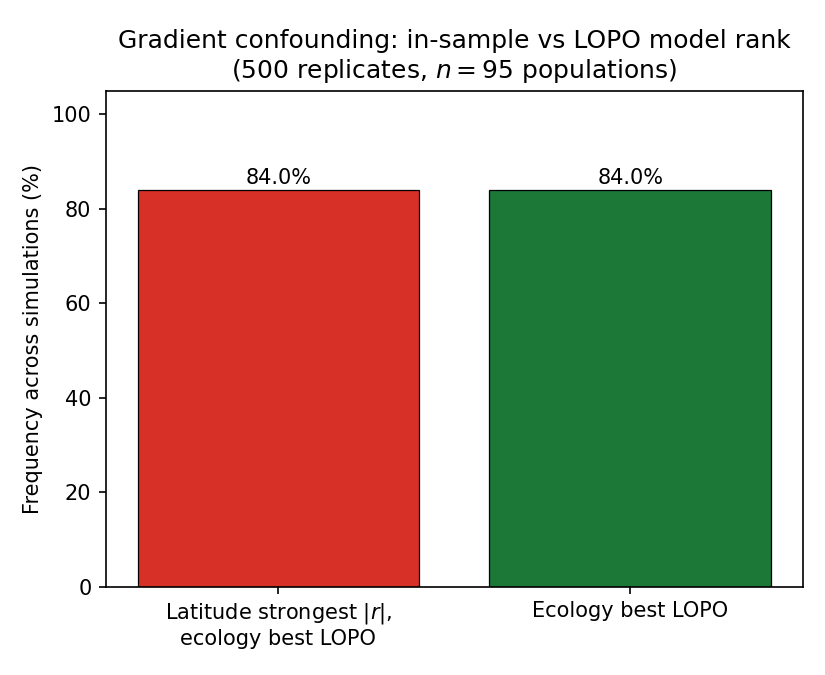
\includegraphics[width=0.72\linewidth]{outputs/figures/simulation_lopo_mismatch_rates.png}
  \end{center}
  \caption{Semi-synthetic validation ($500$ replicates).  In-sample best
    univariate correlate (latitude) mis-ranks models vs.\ LOPO in 84\% of
    replicates under known ecology-driven generating structure.}
  \label{fig:sim-mismatch}
\end{figure}

\paragraph{Geographic cline reanalysis.}
On \emph{Stator limbatus} (Stillwell et al.\ 2007; $n=93$ matched
populations), ecology multivariate achieved LOPO RMSE \textbf{0.104}
versus temperature-only \textbf{0.112} ($-$7.7\% relative); latitude had
the strongest in-sample $|r|$ (0.416) but did not minimise holdout error
(Table~\ref{tab:stator-lopo}).  Individual 10-fold CV inflated ecology
RMSE by ${\sim}$45\% (0.150 vs 0.104), illustrating
Theorem~\ref{prop:estimand-cv-mismatch}
(Table~\ref{tab:cv-unit}).  The 2008 selection experiment failed the
Large$\times$Cold interaction required by a thermal-Bergmann mechanism
\citep{stillwell2008} (Theorem~\ref{prop:two-test}).

\begin{figure}[t]
  \begin{center}
  \fbox{\parbox{0.88\linewidth}{\centering\vspace{2mm}
    \textbf{Figure 2 placeholder} --- composite panel: Table~\ref{tab:stator-lopo}
    (LOPO ranks) + Table~\ref{tab:cv-unit} (CV-unit mismatch).\\[1mm]
    \scriptsize Replace with multi-panel figure at submission.\vspace{2mm}}}
  \end{center}
  \caption{Empirical validation on \emph{S.\ limbatus} geographic survey:
    proxy correlates vs.\ LOPO holdout (2007 survey) and estimand mismatch
    between individual $k$-fold and population LOPO.}
  \label{fig:empirical-summary}
\end{figure}

\begin{table}[t]
  \caption{\emph{Stator limbatus} (2007): in-sample $|r|$ vs LOPO on
    matched populations ($n=93$).}
  \label{tab:stator-lopo}
  \begin{center}
  \begin{tabular}{lccc}
    \toprule
    Model & In-sample $|r|$ & LOPO RMSE & LOPO $R^2$ \\
    \midrule
    Latitude & 0.416 & 0.106 & 0.121 \\
    Mean annual temperature & 0.219 & 0.112 & 0.009 \\
    Ecology multivariate & --- & \textbf{0.104} & \textbf{0.157} \\
    Temperature + ecology & --- & 0.106 & 0.124 \\
    \bottomrule
  \end{tabular}
  \end{center}
\end{table}

\begin{table}[t]
  \caption{Estimand mismatch: individual 10-fold vs LOPO ($n=93$).}
  \label{tab:cv-unit}
  \begin{center}
  \begin{tabular}{lcc}
    \toprule
    CV scheme & Ecology RMSE & Temperature RMSE \\
    \midrule
    10-fold individual & 0.150 & 0.158 \\
    LOPO population mean & 0.104 & 0.112 \\
    \bottomrule
  \end{tabular}
  \end{center}
\end{table}

% ==================================================================
\section{Discussion}
\label{sec:discussion}
% ==================================================================

\paragraph{The central claim.}
Ecological inference is empirical risk minimization on structured data.
Volume~I formalised \emph{learning} across generations; Volume~II
formalises \emph{generalisation} across space---same geometry, different
axis and failure mode.

\paragraph{What this means for ecology.}
Reporting in-sample $R^2$ or AIC on pooled geographic surveys optimises
\Eone\ or confounded proxies, not \Etwo.  Corollary~\ref{cor:operational-default}
is the actionable output: match holdout unit to estimand before interpreting
Bergmann clines, SDMs, or climate-correlate narratives
\citep{blackburn1999,shelomi2012}.  External mapping studies already show
spatial holdout degrades performance \citep{ploton2020}; our framework
explains \emph{why} as wrong risk functionals under confounding.

\paragraph{What this means for machine learning.}
Geographic data are grouped domain-generalisation benchmarks in the wild
\citep{koh2021}.  Invariant prediction methods \citep{arjovsky2019} target
the same object as Grinnellian support under transfer, but ecology adds
nested units, composite labels (plasticity), and explicit mechanism tests.

\paragraph{Bridge to Volume~I.}
Local adaptation at a site is fine-tuning on a spatial subdomain; range
limits are extrapolation failure; plasticity bias is label noise; trade-offs
across sites are multi-task conflict \citep{stillwell2026a}.

\paragraph{Scope and limits.}
Structured ERM addresses predictive geometry, not conservation ethics or
full causal discovery \citep{pearl2009}.  Linear models and population
means simplify presentation; spatial autocorrelation may require blocked
holdout extensions \citep{roberts2017,legendre1993}.

\paragraph{Open problems.}
Optimal block size; invariant prediction under confounded gradients;
connecting Fisher geometry (Volume~I) to spatial Gaussian processes.

% ==================================================================
\section{Methods}
\label{sec:methods}
% ==================================================================

\paragraph{Simulation.}
500 replicates; $n=95$ populations; generating ecology listed in
\texttt{simulation\_lopo\_confounding.py}; LOPO via leave-one-out OLS on
standardised predictors.

\paragraph{Empirical reanalysis.}
Population means from Stillwell et al.\ (2007); LOPO and bootstrap
protocol in Project~50 \citep{stillwell2026methods}.  Code:
\texttt{scripts/simulation\_lopo\_confounding.py}.

% ==================================================================
\appendix
\section{Extended Proofs (Electronic Supplementary Material)}
\label{app:proofs}
% ==================================================================

\subsection{Theorem 1 (Estimand--CV mismatch)}

Individual $k$-fold places test and training individuals at the same
$\mathbf{x}_p$, targeting \Eone\ with extra
$\mathrm{Var}(\varepsilon_{ip}\mid p)$.  LOPO targets \Etwo.

\subsection{Theorems 2--3 (Confounding and rank reversal)}

Omitted-variable bias along collinear $\boldsymbol{\phi}(g)$; constructive
simulation realisation in Section~\ref{sec:empirical-validation}.

\subsection{Theorem 4 (Support bound)}

Lipschitz triangle inequality around nearest point in
$\mathcal{S}_{\mathrm{train}}$.

% ==================================================================
\acks{%
\textbf{Funding:} No external funding was received.

\textbf{Competing Interests:} None declared.

\textbf{Data and code:} Simulation code in Project~55; LOPO reanalysis
protocol in Project~50 \citep{stillwell2026methods}.}

% ==================================================================
\bibliography{stillwell2026b}

\end{document}
